\documentclass[12pt]{article}
% Load packages
\usepackage{url}  % Formatting web addresses
\usepackage{ifthen}  % Conditional
\usepackage{multicol}   %Columns
\usepackage[utf8]{inputenc} %unicode support
\usepackage{amsmath}
\usepackage{amssymb}
\usepackage{epsfig}
\usepackage{epstopdf}
\usepackage{graphicx}
\usepackage[margin=0.1pt,font=footnotesize,labelfont=bf]{caption}
\usepackage{setspace}
%\usepackage{longtable}
\usepackage{colortbl}
%\usepackage{palatino,lettrine}
%\usepackage{times}
%\usepackage[applemac]{inputenc} %applemac support if unicode package fails
%\usepackage[latin1]{inputenc} %UNIX support if unicode package fails
\usepackage[wide]{sidecap}
%\usepackage[authoryear,round,comma,sort&compress]{natbib}
\usepackage[square,sort,comma,numbers,sort&compress]{natbib}
%\usepackage[authoryear,round]{natbib}
\usepackage{supertabular}
\usepackage{simplemargins}
\usepackage{fullpage}
\usepackage{comment}
\usepackage{lineno}
%\usepackage{chicago}
\usepackage{textcomp}
\usepackage{multirow}
\usepackage{amsmath}
\usepackage[linesnumbered,lined,boxed,commentsnumbered]{algorithm2e}
\DeclareMathOperator*{\argmin}{\arg\!\min}

\usepackage{algorithm2e}
\usepackage{algpseudocode}
%\usepackage[space]{cite}
\urlstyle{rm}

%\textwidth = 6.50 in
%\textheight = 9.5 in
%\oddsidemargin =  0.0 in
%\evensidemargin = 0.0 in
%\topmargin = -0.50 in
%\headheight = 0.0 in
%\headsep = 0.25 in
%\parskip = 0.15in
%\linespread{1.75}
\doublespace

%\bibliographystyle{chicago}
\bibliographystyle{plos2009}

\makeatletter
\renewcommand\subsection{\@startsection
	{subsection}{2}{0mm}
	{-0.05in}
	{-0.5\baselineskip}
	{\normalfont\normalsize\bfseries}}
\renewcommand\subsubsection{\@startsection
	{subsubsection}{2}{0mm}
	{-0.05in}
	{-0.5\baselineskip}
	{\normalfont\normalsize\itshape}}
\renewcommand\section{\@startsection
	{subsection}{2}{0mm}
	{-0.2in}
	{0.05\baselineskip}
	{\normalfont\large\bfseries}}
\renewcommand\paragraph{\@startsection
	{paragraph}{2}{0mm}
	{-0.05in}
	{-0.5\baselineskip}
	{\normalfont\normalsize\itshape}}
\makeatother

%Review style settings
%\newenvironment{bmcformat}{\begin{raggedright}\baselineskip20pt\sloppy\setboolean{publ}{false}}{\end{raggedright}\baselineskip20pt\sloppy}

%Publication style settings

% Single space'd bib -
\setlength\bibsep{0pt}

\renewcommand{\rmdefault}{phv}\renewcommand{\sfdefault}{phv}
\newcommand{\norm}[1]{\left\lVert#1\right\rVert}

% Change the number format in the ref list -
\renewcommand{\bibnumfmt}[1]{#1.}

% Change Figure to Fig.
\renewcommand{\figurename}{Fig.}

% Begin ...
\begin{document}
\begin{titlepage}
{\par\centering\textbf{\Large {Modified Flux Balance Analysis}}}
\vspace{0.05in}
{\par \centering \large{ Wei Dai, and Jeffrey D. Varner$^{*}$}}
\vspace{0.10in}
{\par \centering {School of Chemical and Biomolecular Engineering}}
{\par \centering {Cornell University, Ithaca NY 14853}}
\vspace{0.1in}
{\par \centering \textbf{Running Title:}~Modified Flux Balance Analysis}
\vspace{0.1in}
{\par \centering \textbf{To be submitted:}~\emph{Biotechnology~Journal}}
\vspace{0.5in}
{\par \centering $^{*}$Corresponding author:}
{\par \centering Jeffrey D. Varner,}
{\par \centering Professor, School of Chemical and Biomolecular Engineering,}
{\par \centering 244 Olin Hall, Cornell University, Ithaca NY, 14853}
{\par \centering Email: jdv27@cornell.edu}
{\par \centering Phone: (607) 255 - 4258}
{\par \centering Fax: (607) 255 - 9166}
\end{titlepage}
\date{}
\thispagestyle{empty}
\pagebreak
%%%%%%%%%%%%%%%%%%%%%%%%%%%%%%%%%%%%%%%%%%%%%%%%%%%%%%%%%%%%%%%%%%%%%%%%%%%%%%%%%%%%%%%%%%%%%%%%%%%%%%%%%%%
%%%%%%%%%%%%%%%%%%%%%%%%%%%%%%%%%%%%%%%%%%%%%%%%%%%%%%%%%%%%%%%%%%%%%%%%%%%%%%%%%%%%%%%%%%%%%%%%%%%%%%%%%%%
\section*{Abstract}
The use of computational tools and mathematical modeling has long contributed to our understanding of biochemical networks, in particular, there is a long history of quantitative mechanistic modeling. Currently, there are many existing mathematical approaches to characterize biochemical networks such as cellular metabolism and its regulation. However, many of these methods require detailed kinetic and concentration information that are difficult or even impossible to obtain. In the post-genomics era, large-scale stoichiometric reconstructions of microbial metabolism popularized by static, constraint-based modeling techniques such as flux balance analysis (FBA) have become standard tools. However, FBA models assume a pseudo-steady-state (QSS) approximation and cannot account for the intracellular dynamics of the network. Towards those unmet needs, we present a versatile next-generation flux balance analysis model that is capable of capturing intracellular dynamics and concentrations of the network. The access to intracellular information created allowed us to implement preexisting regulatory methods that could not have been done with previous FBA models. The key innovation of our approach is the integration of kinetic-like constraints that work in combination with the objective function to overcome the issues with unidentifiable parameters or mechanisms to predict flux distributions. We tested our approach by modeling dynamic time evolution of two proof-of-concept networks and an E. coli central metabolism network. We were able to replicate classically expected gene expression and enzyme kinetic behavior, including diauxic growth phenomenon. While only small-scale networks with simplified gene expression were evaluated, the framework presented here could be an important first step towards modeling large biochemical networks with undetermined mechanisms or parameters, and complex regulation.


%We further tested the predictive power of the coagulation model parameters against data not used in training, and found good agreement between simulations and experimental measurements. Lastly, we tested the performance of DOPS on commonly used test functions for global optimization and on published biochemical parameter estimation benchmark problems. For the wide range of problems that we considered, DOPS outperformed other meta-heuristic approaches despite a limited number of function evaluations.

\vspace{0.1in}
{\noindent \textbf{Keywords:}~Biochemical engineering, systems biology, flux balance analysis}

% Extra abstract
% Mathematical modeling of biological systems with multiple feed back loops is one such area where parameter estimation is a difficult non-linear optimization problem. This difficulty is further compounded when dealing with parameter vectors of high dimensions.

%In this study, we present the dynamically dimensioned particle
%a novel meta-heuristic approach that combines a variant of particle swarm optimization (PSO) along with dynamically dimensioned search (DDS) to obtain near optimal solutions of high dimensional biochemical networks within a relatively few function evaluations.
%We use a particle swarm optimization technique that uses multi-swarms to generate candidate vectors which are then greedily updated using DDS by dynamically varying the perturbed parameter dimensions. We tested this algorithm (25 trials with 4000 function evaluations in each trial) on a biochemical network of coagulation (148 parameters and 92 species) and compared it's performance against other meta-heuristics like Differential Evolution (DE), Particle Swarm Optimization (PSO), Simulated Annealing (SA) and also against DDS alone. The new algorithm outperforms all the other meta-heuristics on the coagulation model. The parameter vectors obtained using this approach fit the experimental data well and also make accurate enough predictions on unseen experimental data. We also performed this comparison on commonly used test functions (Ackley and Rosenbrock) for global optimization and found the same behavior. Further we used two recently published benchmark problems, a genome wide kinetic model with 1759 parameters and a metabolic model of Chinese Hamster Ovary cells with 117 parameters to evaluate the performance of our approach. We  surprisingly performed well on these benchmarks and obtained the nominal parameter vector with just 4000 function evaluations in both cases.


\pagebreak

\setcounter{page}{1}

% Uncomment in production -
%\linenumbers


\section*{Introduction}

The use of computational tools and mathematical modeling has long contributed to our understanding of biochemical networks, in particular, there is a long history of quantitative mechanistic modeling [1]. Currently, there are many existing mathematical approaches to characterize biochemical networks such as cellular metabolism and its regulation [2-12]. However, many of these methods require detailed kinetic and concentration information that are difficult or even impossible to obtain. Even with the growing data bases for cellular components and development of new reduced order modeling approaches [13], the applications of many mechanistic modeling methods are limited by the lack of kinetic and concentration information. 

To overcome the lack of kinetic information, alternative course-grained modeling approaches have been used to study flux distributions of metabolic networks. In the post-genomics era, large-scale stoichiometric reconstructions of microbial metabolism popularized by static, constraint-based modeling techniques such as flux balance analysis (FBA) have become standard tools [14]. Since the first genome-scale reconstruction of Escherichia coli MG1655 by Edwards and Palsson [15], the reconstruction of over 100 organisms followed [16]. These organisms included prokaryotes such as E. coli [17] or $\mathcal{B}$. subtilis [18] were highly sought after in bioprocessing to maximize yields of desired products. More recently, network reconstructions have been completed on humans as well [19-21]. FBA is a course-grained model that relies on a pseudo-steady-state assumption to reduce unidentifiable kinetic models into an underdetermined linear algebraic system that can be solved efficiently even for large systems. Traditionally, FBA models have lack descriptions of metabolic regulation and control mechanisms that cells need for adapting to different chemical and environmental stimulus. The FBA models instead chooses pathways in the network by prescribing an objective function on metabolism. The use of an objective function is crucial for FBA models since predictions are highly dependent on the objective function used for the analysis. Common objective functions include maximizing growth [14,22-25], ATP production [26], and the production of desired products [27]. The utilization of objective function in FBA models is a huge advantage over mechanistic models because with little to no kinetic parameters, the maximization of biomass production allows for a wide range of predictions that are consistent with experimental observations for microbial systems [14,22,28-33].

In the last decade, FBA have increased in accuracy and utility by incorporating additional biological knowledge from regulatory constraints, thermodynamics, and alternative classes of objective functions [34]. The second generation FBAs initially approached regulatory constraints as Boolean logic operators [31] that arise based on environmental cues. Palsson and coworkers took a bioinformatics approach and incorporated transcription and translation through the use of the E-Matrix to regulate the metabolism [35]. Meanwhile other second generation FBA models focused on incorporating constraints at a physiological level through the use of crowding constraints, enzyme solubility, or membrane economics that constrain the upper limit on the sum of certain or all the flux vectors to increase accuracy of metabolic models [36-38]. The accuracy of the prediction from constraint-based models such as FBA is based heavily on the constraints implemented to reduced the solution space. Second generation FBAs introduce additional constraints that reshape and reduce the solution space to redirect the flux distribution guided by the objective function in a way that more accurately describe biological behaviors. 

In this study, we present an effective biochemical network modeling framework for the construction of a next-generation flux balance analysis. The key innovation of our approach is the integration of kinetic-like constraints that work in combination with the objective function to overcome the issues with unidentifiable parameters or mechanisms to predict flux distributions. These kinetic-like constraints are adjustable parameters that are governed by the presence any combination of: substrate, enzyme, and signaling molecules. This integration allows the description of fluxes and complex regulatory interactions such as allosteric regulation of enzyme activity in the absence of specific kinetic and mechanistic information which limited traditional FBA models. We adopted the regulatory rules and method from [12], which do not rely on overarching theoretical abstractions or restriction assumptions. We tested our approach by modeling the time-evolution of a hypothetical proof-of-concept metabolic network using discretized mass balances. In particular, we verified that our new modeling approach can replicate classically expected gene expression and enzyme kinetic behavior, and capture intracellular metabolite concentrations and regulatory behaviors. Towards these questions, we constructed a proof-of-concept metabolic network that has two enzyme-dependent reactions. In the absence of the specific enzymes, the reactions will not occur, a behaviors that were   that were not captured by the traditional FBA models. We found that our next-generation FBA method has the potential to incorporate gene expression, complex regulatory interactions, and capture intracellular metabolite concentration. Lastly, we tested this framework with a central carbon network for E. coli and was able to adjust minimal parameters to fit experimental data of [39] and capture the diauxic effect of carbon utilization. However, with minimal experimental measurements and known parameters, this modeling approach fails to capture intracellular metabolites at an adequate level. However, we believe that this framework presented here could be an important addition to the next-generation FBA models. 

%The introduction has three paragraphs (introduction no longer than 3 pages):
%\begin{enumerate}
	%\item{\textbf{First~paragraph}: Introduce flux balance analysis as the state of the art in modeling metabolism. }
	%\item{\textbf{Second~paragraph}: Introduce metabolic channeling, both natural and man-made examples. Reference Conrado study, Conrado review, and newer experimental studies in this area.}
%	\item{\textbf{Third~paragraph}: In this study, [Repeat the abstract with some additional detail]. Taken together, [killer statement].}
%\end{enumerate}

% Extra text from the introduction -
%With the capacity to construct very large models using various mathematical formalisms \cite{chen2009input,tasseff2011modeling,luan2007computationally,mo2007genome,orth2011comprehensive,karr2012whole,buchel2013path2models,smallbone2010towards}, more often than not,

%this algorithm (25 trials with 4000 function evaluations in each trial) on a biochemical network of coagulation (148 parameters and 92 species) and compared it's performance against other meta-heuristics  The new algorithm outperforms all the other meta-heuristics on the coagulation model. The parameter vectors obtained using this approach fit the experimental data well and also make accurate enough predictions on unseen experimental data. We also performed this comparison on  and found the same behavior. Further we used two recently published benchmark problems, a genome wide kinetic model with 1759 parameters and a metabolic model of Chinese Hamster Ovary cells with 117 parameters to evaluate the performance of our approach. We  surprisingly performed well on these benchmarks and obtained the nominal parameter vector with just 4000 function evaluations in both cases.
%took into cognizance the fact that it may not be necessary to obtain the exact solution for high dimensional biological systems and that good enough solutions can be quickly obtained without expending a lot of objective function evaluations. Hence our current approach uses the power of population based heuristics along with DDS to obtain near optimal or good solutions. Though in theory we can combine any meta-heuristic with DDS, for the current purpose we used Particle Swarm Optimization (PSO). PSO unlike Genetic Algorithm (GA) or Differential Evolution (DE) does not have complex operations like cross over, mutation or recombination. It is simple to use and does not have a lot of parameters associated with other heuristics. However PSO is known to rapidly converge to a local optimum and thus several variants \cite{peer2003using,zhan2009adaptive,li2007fast} have been developed of which Multi swarm particle swarm optimization approaches (MLSPSO) \cite{zhao2008dynamic,liang2005dynamic} are one of the effective ones. We used MLSPSO to preclude bad regions of search and thereafter search within these regions using DDS.

\clearpage

\section*{Results}

%The results are presented in \textbf{past~tense}. Each paragraph starts with a statement of the result in that paragraph in active voice.
%Each results paragraph ends with a Taken together type statement followed by a link statement e.g., Next we considered etc. When referring to figures, state what the figures shows (Fig. ZZ).

\subsection*{1. Formulation of Proof-of-concept Network Model}

We developed a proof-of-concept metabolic network (Fig. \ref{fig1-schematic}) to investigate the features of our effective biochemical network modeling approach. This ultra-reduced network incorporates metabolic reactions, gene expression, enzyme-dependent reactions, and allosteric regulation. The two examples presented results in the consumption and utilization of an extracellular substrate $\mathcal{A}_{xt}$ in a series of metabolic reactions. Several of these reactions or fluxes involved are enzyme or initiator-dependent. The fluxes that were not explicitly enzyme-dependent assumed enzyme saturation and that the flux is only a function of substrate concentration. 

The conversion from $\mathcal{A}$ to $\mathcal{B}$, and the extracellular uptake of $\mathcal{C}_{xt}$ is dependent on the presence of $enzyme$ $\mathcal{E}$, and $\mathcal{C}$ transporter ($\mathcal{CT}$), respectively. The expression of E and $\mathcal{CT}$ is regulated at the gene expression level. Gene 1 is transcribed and translated into $enzyme$ $\mathcal{E}$ in the presence of growth factors, while Gene 2 transcription and translation results in $\mathcal{CT}$ in a similar manner at a lower concentration of $\mathcal{A}_{xt}$. In the presence of a growth factor that acts as an inducer, the gene for $enzyme$ $\mathcal{E}$ will activate and facilitate transcription and translation reactions to synthesize $enzyme$ $\mathcal{E}$. Meanwhile, in the presence of $\mathcal{A}_{xt}$, the gene expression of is $\mathcal{CT}$ repressed. Once the extracellular $\mathcal{A}$ is depleted, the $\mathcal{C}$ transporter will be synthesized. In our formulation, Hill-like transfer functions were used to calculate the influence of factor abundance on target enzyme activity. In this context, factors can be a function of metabolite concentration or flux. The kinetic-like constraints are multiplied by an activity control between 0 and 1. 

Gene expression in the proof-of-concept network involved is a two-step process: transcription and translation. The course-grained transcription and translation reactions in our network neglected the utilization of NTPs and amino acids. Transcription in the proof-of-concept network is solely determined by the presence of the relevant inducer, respective gene, and RNA polymerase concentration, and translation reactions were determined by mRNA and ribosome concentration. We assumed the generation of RNA polymerase and ribosome synthesis to be a zeroth order constant while degradation to be a first order rate. 

A critical test of our modeling approach was to simulate networks with known behavior. If we cannot reproduce the expected behavior of simple networks, then our effective modeling strategy and particular rules of constraining fluxes will not be feasible for large-scale networks. We considered two cases that had identical initial concentrations and kinetic parameters but with different objective functions and gene expression. The first case involved the synthesis of $\mathcal{B}_{xt}$ from $\mathcal{A}_{xt}$, a case analogous to the maximization of a desired product while minimizing any undesired byproducts. The second case we tested included the addition of a biomass template reaction and we explored the diauxic growth phenomenon through a simplified representation of carbon catabolite repression. 

\subsection*{1.1 Dynamics of inducers and enzyme dependent reactions}

The following study focused on the impact of growth factor (inducer) on networks aimed at the production of $\mathcal{B}_{xt}$. Metabolic Gene 2 (Fig. \ref{fig1-schematic}) responsible for the expression of $\mathcal{CT}$ was not included. The growth factor concentration was varied systematically in a linear fashion and the dynamic changes in system was determined. We implemented the objective function to maximize the production of $\mathcal{B}_{xt}$. The intracellular metabolites concentrations were constrained with a lower limit of zero while the flux bounds were implemented as a function of substrate concentration, control parameters, and enzyme concentration for the reactions that were enzyme dependent. The biomass was kept at a constant of 0.1 gDW/L without any growth. Gene expression of $enzyme$ $\mathcal{E}$ was governed by the concentration of the inducer, a growth factor. With the increased inducer concentrations, we observed an expected increase in mRNA and enzyme concentration until steady state (Fig. \ref{fig2-nogrowth}A). 

The presence of Enzyme E facilitated the conversion of $\mathcal{A}$ to $\mathcal{B}$. The rate of conversion was governed by the concentration of both of the Enzyme E and species $\mathcal{A}$. The rate of conversion of $\mathcal{A}$ to $\mathcal{B}$ is shown in Fig. \ref{fig2-nogrowth}B. At an inducer concentration of zero, the rate of conversion is zero (not shown). Initially, the rate of $\mathcal{A}_{xt}$ uptake was greater than the consumption of species $\mathcal{A}$ (Fig. \ref{fig2-nogrowth}C). As $enzyme$ $\mathcal{E}$ accumulated, the conversion of $\mathcal{A}$ to $\mathcal{B}$ increased proportionally to $enzyme$ $\mathcal{E}$’s and substrate $\mathcal{A}$’s concentration. The total rate of consumption $\mathcal{A}$ was greater than the generation, causing it to deplete until intracellular $\mathcal{A}$ reaches steady state. 

The gene expression of $enzyme$ $\mathcal{E}$ redirected the pathway of synthesis for product $\mathcal{B}_{xt}$. In the absence of of $enzyme$ $\mathcal{E}$, $\mathcal{B}$ can only be formed from the longer path of conversion of $\mathcal{A}$ to$\mathcal{C}$ to $\mathcal{B}$ (Fig. \ref{fig1-schematic}). This pathway leads to an increased production of undesired  byproduct $\mathcal{C}_{xt}$ (Fig. \ref{fig2-nogrowth}D). The presence of Enzyme E opens a new pathway for the direct synthesis of $\mathcal{B}_{xt}$ through the conversion of $\mathcal{A}$ to $\mathcal{B}$ (Fig. \ref{fig1-schematic}) and reduces the accumulation of intracellular$\mathcal{C}$ and byproduct $\mathcal{C}_{xt}$ (Fig. \ref{fig2-nogrowth}D). 


\subsection*{1.2 Dynamics of Growth and Alternative Substrate Utilization}

The proof-of-concept network was used to test whether our approach is capable of capturing the diauxic growth phenomenon observed in bacteria using gene expression to regulate the metabolism. A biomass template reaction of intracellular metabolite consumption was constructed:
\begin{equation}\label{eq:static_opt}
\begin{aligned}
2 \mathcal{A} + \mathcal{B} + \mathcal{C} \rightarrow Biomass
\end{aligned}
\end{equation} 
The growth factor that is responsible for the expression of $enzyme$ $\mathcal{E}$ which catalyzes the conversion of $\mathcal{A}$ to $\mathcal{B}$ was maintained constant at zero. The objective function was implemented to maximize biomass production and the species and flux constraints were implemented the same way as the previous case. 

We used an initial biomass concentration of 0.1 gDW/L, and a growth rate constraint set between  to initiate the simulation with 10 arbitrary units of $\mathcal{A}_{xt}$. The extracellular product, $\mathcal{C}_{xt}$ is generated as a byproduct from the production of all the biomass precursors (Fig. \ref{fig3-growth}A) since the presence of species$\mathcal{C}$ drives the flux of$\mathcal{C}$ to $\mathcal{C}_{xt}$. As $\mathcal{A}_{xt}$ is depleted, the repression of $\mathcal{CT}$ gene expression decreases gradually in a sinusoidal behavior with respect to $\mathcal{A}_{xt}$ concentration. When all of the $\mathcal{A}_{xt}$ was consumed, gene expression of $\mathcal{CT}$ became uninhibited and the production of $\mathcal{CT}$ allowed the network to uptake $\mathcal{C}_{xt}$ and utilize it as an alternate substrate for growth (Fig. \ref{fig3-growth} $\mathcal{A}$ and B).

With the proof-of-concept model, we were able to capture the diauxic growth phenomenon with regulation at the level of gene expression. We witnessed a decrease in intracellular species concentration due to the decreasing substrate uptake rate relative to the metabolic demand of growth. However, when $\mathcal{A}_{xt}$ was depleted, intracellular $\mathcal{B}$ and$\mathcal{C}$ began to accumulate due to the relatively high $\mathcal{C}_{xt}$ uptake rate compared to that of $\mathcal{A}_{xt}$ uptake rate before complete depletion. As $\mathcal{C}_{xt}$ was consumed, the intracellular concentrations decreased again (Fig. \ref{fig3-growth}D). 

In addition, we witnessed that the intracellular concentration of $\mathcal{B}$ depleted rapidly due to biomass demand (Fig. \ref{fig3-growth}D). Species $\mathcal{B}$ is synthesized by the conversion from C, and is consumed by the conversion of $\mathcal{B}$ to $\mathcal{A}$ and biomass synthesis, and diluted due to growth. Intracellular $\mathcal{B}$ is the last species in the linear pathway (Fig. \ref{fig3-growth}E), the mFBA is optimized to only provide enough $\mathcal{B}$ for growth and dilution which kept the $\mathcal{B}$ concentration at minimal. Once $\mathcal{A}_{xt}$ is depleted, $\mathcal{B}$ accumulated and facilitated the conversion of $\mathcal{B}$ to $\mathcal{A}$ to provide the biomass demand for $\mathcal{A}$. $\mathcal{A}$ is the last species in the linear pathway, similarly, $\mathcal{A}$ concentration became minimal. Our method was able to reduce the solution space, successfully capturing complex trends by using simple Hill function and kinetic-like constraints.

\subsection*{1.3 Initialization of E. coli Diauxic model}

As stated before, a critical test of our modeling approach was to simulate networks with known behavior. We decided to implement our framework on the central carbon metabolism of E. coli. In addition, we wanted to test the potential of our modeling approach when the kinetic parameters, mechanistic equations, and regulatory effects within the network architecture were not known. We formed simple regulatory rules based on observation of the experimental data [39] of diauxic growth: the uptake of acetate was inhibited at high levels of glucose uptake. Our E. coli model, consist of 65 species and 111 reactions including the template biomass reaction adopted from [41] (Fig. \ref{fig4-Ecoli}A). For the initialization of intracellular metabolite concentration, we used measured values from different literature sources [41,42]. For the kinetic-like flux constraints, we decided to implement the classic Michaelis Menten (MM) kinetics to capture any saturation effects within the system since the metabolite concentration are well above saturation in vivo [41].

A critical challenge for any dynamic ODE model is the estimation of kinetic parameters. For metabolic processes, there is also the added challenge of identifying the regulation and control structures that manage metabolism. This problem still exists with our FBA modeling approach, but this challenge can be overcome by increasing the uncertainty of our kinetic-like flux constraints. By doing so, the distance between the upper and lower flux increased and therefore increase the solution space and the optimized solution becomes more heavily influenced by the objective function. In our system, we decided to take a course-grained approach for parameter estimation to test the capacity and adaptability of our modeling framework. Using our course-grained parameter estimation approach, the Michaelis Menten parameter were evaluated based on the initial condition of the cellular system. $\mathcal{A}$ standard FBA was then carried out, optimizing for growth rate. The calculated solution to the fluxes was used to evaluate Vmax using initial substrate concentrations and assuming a Km of 1/50 of the species’ initial concentration. For pathways that were not utilized, ie flux of zero, in the standard FBA solution, the flux constraints were unbound due to the uncertainty. To account for the error and uncertainty associated with this crude estimation, an uncertainty tolerance was placed between the lower and upper bound as a constraint that the flux value must fall within. To determine this variation within the flux constraint, we varied a global parameter across all flux constraints that were governed by MM to fit experimental data. Most of the fluxes in our system were not sensitive to the change solution space. In most metabolic networks, only a few reactions are rate limiting and act as a bottleneck for the whole system. Increasing the solution space did not impact the fluxes downstream of the bottleneck. This robustness within our system is similar to the findings of Sethna and coworkers who indicate that the model’s performance is often controlled by only a few parameter combinations, a characteristic that seems universal for multi-parameter models referred to as sloppiness [43]. Regulatory control was put in place for the uptake of acetate by utilizing a Hill-function governed by the flux of glucose uptake rate of the previous iteration of the discretized mass balance. The parameters in the fill functions were determine by manually fitting against experimental data. The pathways of gluconeogenesis shown in Fig. \ref{fig4-Ecoli}A were not regulated, but rather controlled by the optimization from the objective function. 

Under the assumed condition, our model was able to accurately capture experimental measurements of extracellular glucose and acetate, and the biomass and glucose-acetate diauxie phenomenon (Fig. \ref{fig4-Ecoli}B). However due to the crude parameter estimation, some dynamic resolution of the intracellular concentration were lost. Most of the intracellular metabolites either accumulated or depleted to the concentration limits that were set for the intracellular species. On closer examination, the two intracellular byproducts of growth, formate and acetate (Fig. \ref{fig4-Ecoli}A), accumulated towards their respective concentration threshold. However, formate depleted rapidly, reaching it’s lower threshold concentration after it reached the maximum threshold concentration. Upon the depletion of glucose, the state of the system changed to the utilization of acetate leading to a new set of flux distribution. The flux of the glycolysis and gluconeogenesis are shown in Fig. \ref{fig4-Ecoli}D. The flux of the glycolysis pathway shown remained constant throughout growth with the utilization of glucose, upon glucose depletion, the flux of gluconeogenesis took over in supplying carbon into the upper glycolysis and pentose phosphate pathways for biomass precursor production. 






\clearpage

%As the dimensionality of  increases, the search region gets widened and thus the problem becomes more challenging.
%

\section*{Discussion}

In this study, we presented an effective kinetic-like constraint-based FBA model to dynamically simulate metabolic networks. Our proposed strategy integrated a kinetic modeling approach with an objective function from the traditional FBA to dynamically describe metabolic regulation and control. We tested this model approach by developing a hypothetical proof-of-concept network and a central carbon E. coli network. In particular, we tested whether our effective modeling approach could describe classically expected behaviors through the combination of regulatory control from allosteric regulation and gene expression. Towards these questions, we explored two hypothetical and one realistic networks. In each of the two hypothetical networks, substrate $\mathcal{A}_{xt}$ was transported into the cell and consumed for the production of $\mathcal{B}_{xt}$ or biomass depending on the objective function. The E. coli network consumed glucose for the production of biomass precursors for growth. The reactions were assumed to be only substrate-dependent unless specifically implemented to be a function of substrate and enzyme concentrations. When these flux constraints were integrated into the network models, these constraints captured dynamic patterns in the flux and concentration in the network. Lastly, we implemented this method on a central carbon metabolic network of E. coli, and captured the diauxic growth phenomenon. 

This proposed modeling technique shares features with other modeling techniques. The implementation of the flux constraints is flexible and can take the form of most kinetic or mechanistic forms, ie mass action kinetics or effective kinetic formats [44]. This new modeling approach takes the form of a discretized form of effective kinetic model in the way that flux constraints that are implemented. The overall purpose of our framework functioned in a similar manner as other FBA models to reduce the solution space to what is biologically or thermodynamically relevant. The real innovation of this modeling approach is imploring the use of intracellular metabolite. This subtle difference allowed us to integrate preexisting an effective kinetic modeling approach [12,13] into our kinetic-like constraints. In addition, having access to intracellular species information allowed us to integrate allosteric regulation into the model. 

This proposed modeling framework also differs appreciably from previous established FBA models. The vast difference between our proposed method and an ODE models involves the uncertainty that sets tolerance between the governing kinetic form and the upper and lower bound of the flux constraint and the guidance of the objective function. Even with unidentifiable kinetic parameters, this combination of high uncertainty and objective function of our modeling approach can overcome this problem. Based on the fluxes that were determined, the kinetic parameters of the most optimized flux distribution could be determined and analyzed for feasibility. Unlike the previous FBA models, we did not make the quasi-steady-state (QSS) assumption for intracellular species. Our internal species was allowed to accumulate and deplete at a constant rate each time the discretized mass balances were evaluated so that the intracellular concentrations could be captured and implemented as contributors for allosteric regulation. At high uncertainty of the kinetic parameters, we were still able to effectively capture glucose consumption, growth, and the diauxic phenomenon. Unfortunately, dynamic resolution for intracellular metabolites was lost as most of the intracellular metabolites approached their upper and lower limits. However, with enough certainty in our parameters, we were able to fully capture the dynamics of intracellular metabolite in our proof-of-concept networks. 

In summary, our proposed framework offers an effective method of reducing the solution space of the FBA by using kinetic-like approximations that captured simple enzyme dependence, allosteric regulation, and diauxic growth. At it’s core, our effective modeling approach combines advantages of FBA and kinetic ODE models. The use of an objective function that acts as a global predictor will overcome problems pertaining unidentifiable parameters or mechanisms, meanwhile the use of kinetic-like constraints on the fluxes acts as a local check-points that reshapes the solution space that is closer to the true behavior of the network. There is a trade off between uncertainty and resolution as expected for any model. At the uncertainty of our system increases, our mFBA approaches the state of a tradition FBA where the solution is determined from the objective function. Meanwhile as uncertainty of our system approaches zero, our modeling approach takes a form that is more similar to an ODE model that is discretized and the solution is shaped by kinetic-like flux constraints. We believe that utilization of this modeling approach is for large networks with unidentifiable parameters or unsalable using ODEs.  

%The discussion has three (sometimes four) paragraphs:
%\begin{enumerate}
%	\item{\textbf{First~paragraph}: Present a modified version of the last paragraph of the introduction. In this study, [...]. Taken together, [killer statement]}
%	\item{\textbf{Second~paragraph}: Contrast the key findings of the study with other computational/experimental studies}
%	\item{\textbf{Third~paragraph}: Present future directions. If you had more time, what would like to do? Highlight the key shortcomings of the approach and how will we address them in the future.
%	In this case, we will have a scaling issue if we extend to genome scale. We should extend to dynamic cases, and we need to experimentally validate the findings. }
%\end{enumerate}

\clearpage

\section*{Materials and Methods}

The Modified Flux Balance Analysis (mFBA) is new method created for the study of biochemical networks much like the traditional flux balance analysis. The mFBA utilizes series of species constraints and flux constraints similar to the traditional FBA. The mass balances for each species are discretized and solved using explicit numerical methods such as explicit Euler as in Equations 2 and 3.


\begin{equation}\label{eq:MB1}
\begin{aligned}
\frac{dx}{dt}= \mathcal{S}* v- \mu x=b \\
\end{aligned}
\end{equation}

\begin{equation}\label{eq:MB2}
\begin{aligned}
&Intracellular Species: x_{t+1} = x_t + b\Delta t - x_t \mu \Delta t\\
\end{aligned}
\end{equation}

\begin{equation}\label{eq:MB3}
\begin{aligned}
&Extracellular Species: x_{t+1} = x_t + b\Delta t - x_t \mu \Delta t\\
\end{aligned}
\end{equation}



In equation 2,  is the stoichiometric matrix with m species by n reactions,  is a flux vector of each reaction, denotes the growth rate and  is a vector of change in species with respect to time. In the discretized mass balances, Equations 3a and 3b,  the time, is the growth rate, and  denotes the species concentration. For traditional FBA, the intracellular species (IS) were assumed to be at quasi-steady-state (QSS), making the species constraint, . However, for the mFBA, we assumed an initial concentration for intracellular species concentration based on literature measurements [41,42] and did not assume QSS by allowing intracellular metabolites to accumulate and deplete within a physiological range. By incorporating the lower and upper limit the species concentration and dilution due to growth, the species constraints implemented in our model is shown in Equation 4. 

\begin{equation}\label{eq:SBA}
\begin{aligned}
LB - x(1-\mathbf{dsa}\mu)\le S*v \le UB - x(1-\mathbf{dsa}\mu)
\end{aligned}
\end{equation}
%LB-x(1-dsa \Mu ) 

In Equation 4  and  are vectors of lower and upper limits of each species, while  represents the dilution selection array, a Boolean vector that takes determines whether a species is diluted due to growth, ie. 0 for extracellular species that are not diluted and 1 for intracellular species that are.

The flux constraints use two key components. The kinetics portion are implemented as a function of species concentration in a generalized fashion, and then the regulation portion is incorporated for regulatory mechanisms. The flux is constrained between two a lower and upper bound (Equation 5).
\begin{equation}\label{eq:FB1}
\begin{aligned}
\alpha \le v \le\beta   
\end{aligned}
\end{equation}
For tradition FBA,  and  are a vector of constants same length as the number of reactions, for our modeling approach, they are functions of control parameters, substrate concentration, and/or enzyme concentration as shown in Equation 6:
\begin{equation}\label{eq:FB2}
\begin{aligned}
&\alpha=f_1 (\epsilon)v
&\beta=f_2  (\epsilon)v_k
\end{aligned}
\end{equation}
where and  are uncertainty functions of  , the uncertainty coefficient, a constant that is used to control the solution space in the model based on the certainty in the parameters in the kinetic-like constraints, . The uncertainty functions act as a way to widen the distance between lower and upper limit defined by kinetic-like constraints. The kinetic-like constraints,  can take any form, from mechanistic descriptions to effective kinetic models like the power-law:
\begin{equation}\label{eq:FB3}
\begin{aligned}
v_k= \alpha x^n*C          
\end{aligned}
\end{equation}
where  and  represents vectors of gain coefficients and cooperativity coefficients of the power law respectively. The  vector is a control vector that utilizes Hill-functions to describe any types of regulation within the network for both activation and repression.
\begin{equation}\label{eq:HillFunction}
\begin{aligned}
&Activation: \mathcal{C} = \frac{\beta x^n}{1+\beta x^n}
&Repression: \mathcal{C} = 1 - \frac{\beta x^n}{1+\beta x^n}
\end{aligned}
\end{equation}
Similarly,  and  represents vectors of gain coefficients and cooperativity coefficients.
Lastly, the network is subjected to the objective function, :
\begin{equation}\label{eq:OBJ}
\begin{aligned}
Z = \sum_{i=1}^{n_{fluxes}} c*v
\end{aligned}
\end{equation}
The vector  was used to select a linear combination of metabolic fluxes that were included in the objective function. In our examples, we have defined either production of desired species or cellular growth to be our objective function. 

%\begin{enumerate}
%	\item{\textbf{Model~formulation}: Present the spatial flux balance approach, and enzyme balances for the (un)channeled case. Outline any bounds formulation, and state all parameter assumptions.}
%\end{enumerate}

\clearpage

%Need to talk more about biochemical benefits and importance for of biochemical problems

\section*{Acknowledgements}
This study was supported by an award from [FILL ME IN].
\clearpage


\bibliography{References_v1}

\clearpage

% Figures and captions go here ...
%\begin{figure}[ht]
%\centering
%\includegraphics[width=1.00\textwidth]{./figs/<Filename>.pdf}
%\caption{Captiontext goes here}
%}\label{fig:<label_name>}
%\end{figure}
\clearpage

\begin{figure}[h]
\centering
\includegraphics[width=1.0\textwidth]{./Figures/Figure1_POC_Schematic.pdf}
\caption{Proof-of-concept metabolic network considered in this study. The black arrows indicate depletion and formation, the red arrows indicate repression, the green represents activation, and the grey arrows are enzyme-dependent reactions. Substrate $A_{xt}$ can be transported into the cell and converted into $B$ and $C$ to be transported out. The reactions that are enzyme dependent are subjected to regulation with respect to gene expression ($enzyme$ $\mathcal{E}$ and $C transporter$).
}\label{fig1-schematic}
\end{figure}

\clearpage
\begin{figure}[h]
\centering
\includegraphics[width=1.0\textwidth]{./Figures/Figure2_POC_Nogrowth.pdf}
\caption{ \textbf{(A)}: mRNA E and Enzyme E response for different growth factor concentrations. Inducer concentration of zero did not express any mRNA or Enzyme (not shown). \textbf{(B)}: Flux of $A$ to $B$ catalyzed by $Enzyme E$. The rate of $A$ conversion to $B$ is proportional to the Enzyme E and substrate $\mathcal{A}$ concentration. \textbf{(C)}: Intracellular concentration of $A$. \textbf{(D)}: $C_{xt})$ concentration in the absence of $C transporter$. The production of $C_{xt}$ decreases with increasing growth factor inducer concentration.
}\label{fig2-nogrowth}
\end{figure}

\clearpage
\begin{figure}[h]
\centering
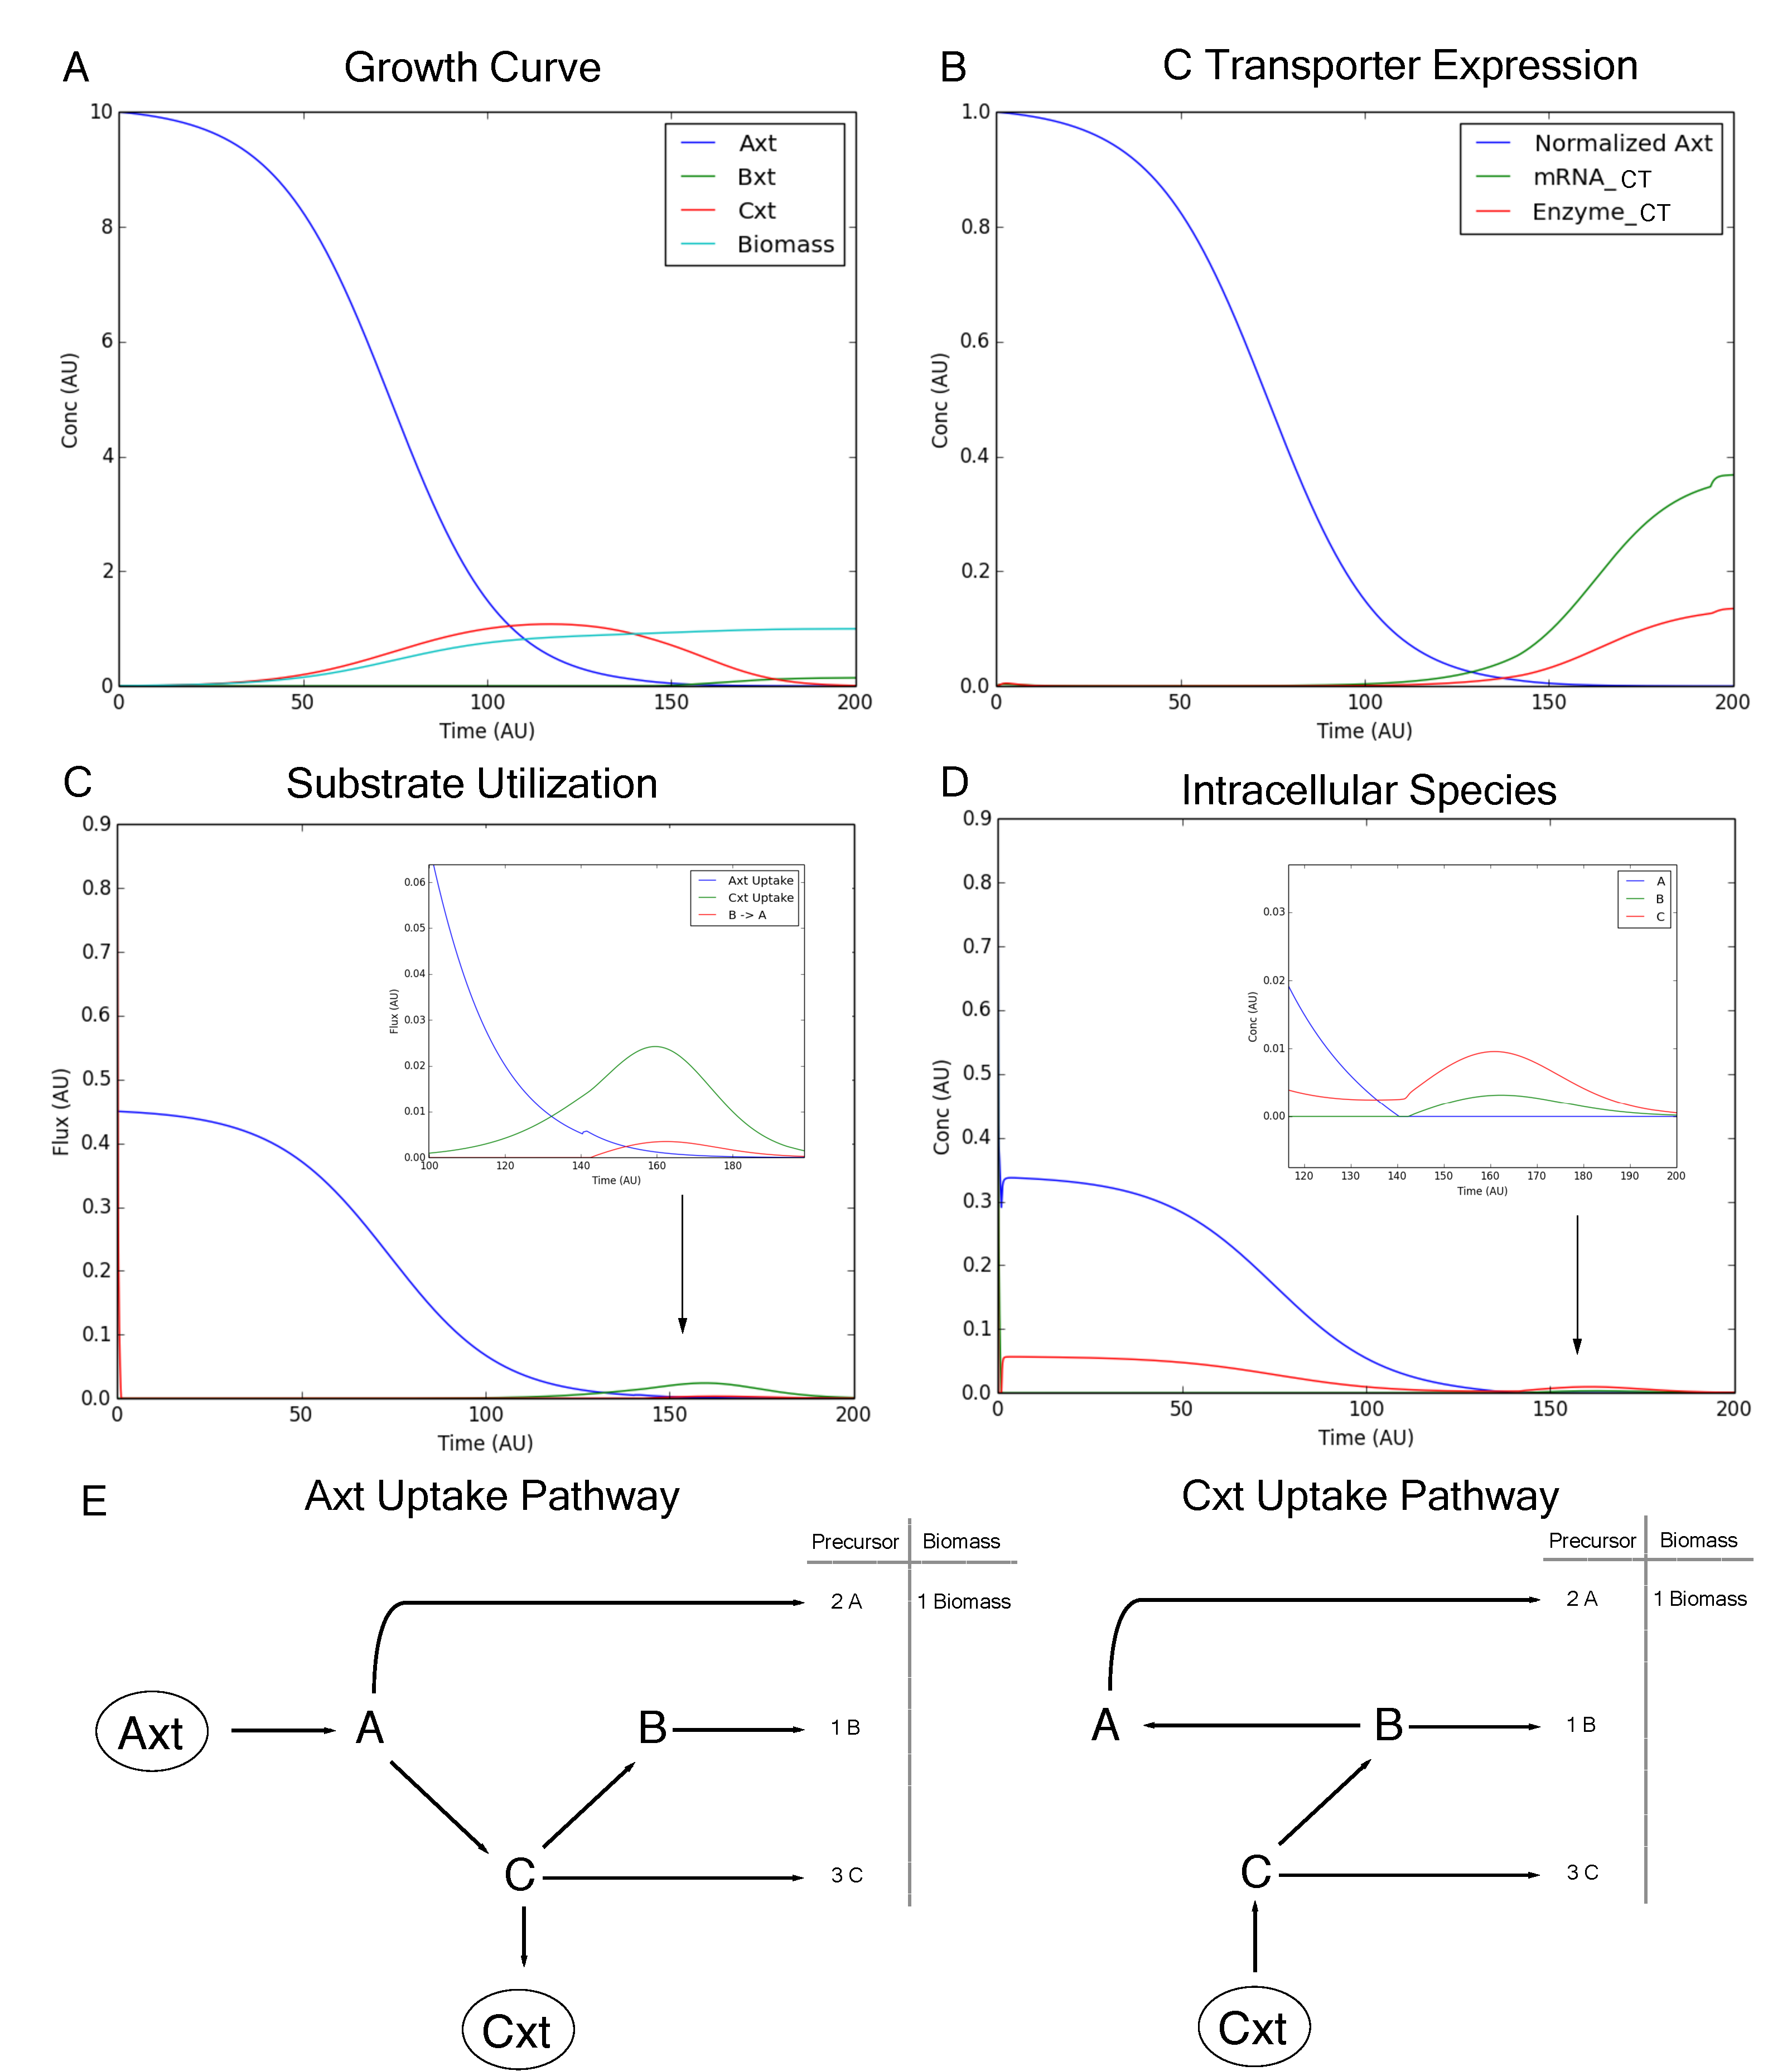
\includegraphics[width=1.0\textwidth]{./Figures/Figure3_POC_Growth.pdf}
\caption{\textbf{(A)}: Growth Curve indicates the utilization of $C_{xt}$ as an alternate substrate when $A_{xt}$ is depleted. \textbf{(B)} Production of mRNA $C transporter$ and $C transporter$ enzyme begins once the $A_{xt}$ concentration is below it’s inhibition threshold concentration. \textbf{(C)}: The conversion of $B$ to $A$ is required for intracellular replenishment for growth upon $A_{xt}$ depletion. \textbf{(D)}: Concentration of intracellular species. \textbf{(E)}: Linear pathway of metabolic flux. While $A_{xt}$ is available, intracellular $A$, $C$ and $B$ are first, second, and third species respectively in the linear pathway. Once $A_{xt}$ is depleted and $C_{xt}$ is utilized as an alternate substrate, the order of the pathway changes to $C$, $B$, and $A$.
}\label{fig3-growth}
\end{figure}

\clearpage
\begin{figure}[h]
\centering
\includegraphics[width=1.0\textwidth]{./Figures/Figure4_Ecoli.pdf}
\caption{\textbf{(A)}: Simplified illustration of the E.coli central metabolism. The red arrows represent the fluxes for gluconeogenesis. \textbf{(B)}: Growth curve showing utilization of acetate compared against experimental measurements from Varma et al [REF]. \textbf{(C)}: Intracellular metabolite concentration of two by products, acetate and formate. \textbf{(D)}: Flux of glycolysis and gluconeogenesis.
}\label{fig4-Ecoli}
\end{figure}

\clearpage

\clearpage

% Supplemental figures -
% Set the S-
\renewcommand\thefigure{S\arabic{figure}}
\renewcommand\thetable{T\arabic{table}}
\renewcommand\thepage{S-\arabic{page}}
\renewcommand\theequation{S\arabic{equation}}

% Reset the counters -
\setcounter{equation}{0}
\setcounter{table}{0}
\setcounter{figure}{0}
\setcounter{page}{1}


% Supplemental figures go here ...
%\begin{figure}[ht]
%\centering
%\includegraphics[width=1.00\textwidth]{./figs/<Filename>.pdf}
%\caption{Captiontext goes here}
%}\label{fig:<label_name>}
%\end{figure}

\end{document}
